%        File: arfc-beamer.tex
%     Created: Sun May 5 10:00 PM 2013 C
%


%\documentclass[11pt,handout]{beamer}
\documentclass[9pt]{beamer}
\usetheme[white]{Illinois}
%\title[short title]{long title}
\title[Short Title]{Optimal Sizing of a Nuclear Reactor for Embedded Grid Systems}
%\subtitle[short subtitle]{long subtitle}
\subtitle[Short SubTitle]{Preliminary Work}
%\author[short name]{long name}
\author[Samuel Dotson]{Samuel G. Dotson\\Advanced Reactors and Fuel Cycles Group}
%\date[short date]{long date}
% \date[05.21.2020]{May 21, 2020}
\date{\today}
%\institution[short name]{long name}
\institute[UIUC]{University of Illinois at Urbana-Champaign}

%\usepackage{bbding}
\usepackage{amsfonts}
\usepackage{amsmath}
\usepackage{xspace}
\usepackage{graphicx}
\graphicspath{{../figures/}}
\usepackage{subfigure}
\usepackage{booktabs} % nice rules for tables
\usepackage{microtype} % if using PDF
\usepackage{bigints}
\usepackage{minted}

\newcommand{\units}[1] {\:\text{#1}}%
\newcommand{\SN}{S$_N$}%{S$_\text{N}$}%{$S_N$}%
\DeclareMathOperator{\erf}{erf}
%I need some complimentary error funcitons...
\DeclareMathOperator{\erfc}{erfc}
%Those icons in the references are terrible looking
\setbeamertemplate{bibliography item}[text]

%%%% Acronym support

\usepackage[acronym,toc]{glossaries}
\newacronym[longplural={metric tons of heavy metal}]{MTHM}{MTHM}{metric ton of heavy metal}
\newacronym{ABM}{ABM}{agent-based modeling}
\newacronym{ACDIS}{ACDIS}{Program in Arms Control \& Domestic and International Security}
\newacronym{AHTR}{AHTR}{Advanced High Temperature Reactor}
\newacronym{ANDRA}{ANDRA}{Agence Nationale pour la gestion des D\'echets RAdioactifs, the French National Agency for Radioactive Waste Management}
\newacronym{APP}{APP}{Abbott Power Plant}
\newacronym{ANL}{ANL}{Argonne National Laboratory}
\newacronym{API}{API}{application programming interface}
\newacronym{ARCH}{ARCH}{autoregressive conditional heteroskedastic}
\newacronym{ARE}{ARE}{Aircraft Reactor Experiment}
\newacronym{ARFC}{ARFC}{Advanced Reactors and Fuel Cycles}
\newacronym{ARMA}{ARMA}{autoregressive moving average}
\newacronym{ASME}{ASME}{American Society of Mechanical Engineers}
\newacronym{ATWS}{ATWS}{Anticipated Transient Without Scram}
\newacronym{BDBE}{BDBE}{Beyond Design Basis Event}
\newacronym{BIDS}{BIDS}{Berkeley Institute for Data Science}
\newacronym{BOL}{BOL}{Beginning-of-Life}
\newacronym{BSD}{BSD}{Berkeley Software Distribution}
\newacronym{CAFCA}{CAFCA}{ Code for Advanced Fuel Cycles Assessment }
\newacronym{CASL}{CASL}{Consortium for Advanced Simulation of Light Water Reactors}
\newacronym{CDTN}{CDTN}{Centro de Desenvolvimento da Tecnologia Nuclear}
\newacronym{CEA}{CEA}{Commissariat \`a l'\'Energie Atomique et aux \'Energies Alternatives}
\newacronym{CI}{CI}{continuous integration}
\newacronym{CNEC}{CNEC}{Consortium for Nonproliferation Enabling Capabilities}
\newacronym{CNEN}{CNEN}{Comiss\~{a}o Nacional de Energia Nuclear}
\newacronym{CNERG}{CNERG}{Computational Nuclear Engineering Research Group}
\newacronym{COSI}{COSI}{Commelini-Sicard}
\newacronym{COTS}{COTS}{commercial, off-the-shelf}
\newacronym{CSNF}{CSNF}{commercial spent nuclear fuel}
\newacronym{CTAH}{CTAHs}{Coiled Tube Air Heaters}
\newacronym{CUBIT}{CUBIT}{CUBIT Geometry and Mesh Generation Toolkit}
\newacronym{CURIE}{CURIE}{Centralized Used Fuel Resource for Information Exchange}
\newacronym{DAG}{DAG}{directed acyclic graph}
\newacronym{DANESS}{DANESS}{Dynamic Analysis of Nuclear Energy System Strategies}
\newacronym{DBE}{DBE}{Design Basis Event}
\newacronym{DESAE}{DESAE}{Dynamic Analysis of Nuclear Energy Systems Strategies}
\newacronym{DHS}{DHS}{Department of Homeland Security}
\newacronym{DOE}{DOE}{Department of Energy}
\newacronym{DRACS}{DRACS}{Direct Reactor Auxiliary Cooling System}
\newacronym{DRE}{DRE}{dynamic resource exchange}
\newacronym{DSNF}{DSNF}{DOE spent nuclear fuel}
\newacronym{DYMOND}{DYMOND}{Dynamic Model of Nuclear Development }
\newacronym{EBS}{EBS}{Engineered Barrier System}
\newacronym{EDZ}{EDZ}{Excavation Disturbed Zone}
\newacronym{EIA}{EIA}{U.S. Energy Information Administration}
\newacronym{EPA}{EPA}{Environmental Protection Agency}
\newacronym{EP}{EP}{Engineering Physics}
\newacronym{FCO}{FCO}{Fuel Cycle Options}
\newacronym{FCT}{FCT}{Fuel Cycle Technology}
\newacronym{FCWMD}{FCWMD}{Fuel Cycle and Waste Management Division}
\newacronym{FEHM}{FEHM}{Finite Element Heat and Mass Transfer}
\newacronym{FEPs}{FEPs}{Features, Events, and Processes}
\newacronym{FHR}{FHR}{Fluoride-Salt-Cooled High-Temperature Reactor}
\newacronym{FLiBe}{FLiBe}{Fluoride-Lithium-Beryllium}
\newacronym{GCAM}{GCAM}{Global Change Assessment Model}
\newacronym{GDSE}{GDSE}{Generic Disposal System Environment}
\newacronym{GDSM}{GDSM}{Generic Disposal System Model}
\newacronym{GENIUSv1}{GENIUSv1}{Global Evaluation of Nuclear Infrastructure Utilization Scenarios, Version 1}
\newacronym{GENIUSv2}{GENIUSv2}{Global Evaluation of Nuclear Infrastructure Utilization Scenarios, Version 2}
\newacronym{GENIUS}{GENIUS}{Global Evaluation of Nuclear Infrastructure Utilization Scenarios}
\newacronym{GPAM}{GPAM}{Generic Performance Assessment Model}
\newacronym{GRSAC}{GRSAC}{Graphite Reactor Severe Accident Code}
\newacronym{GUI}{GUI}{graphical user interface}
\newacronym{HLW}{HLW}{high level waste}
\newacronym{HPC}{HPC}{high-performance computing}
\newacronym{HTC}{HTC}{high-throughput computing}
\newacronym{HTGR}{HTGR}{High Temperature Gas-Cooled Reactor}
\newacronym{IAEA}{IAEA}{International Atomic Energy Agency}
\newacronym{IEMA}{IEMA}{Illinois Emergency Mangament Agency}
\newacronym{INL}{INL}{Idaho National Laboratory}
\newacronym{IPRR1}{IRP-R1}{Instituto de Pesquisas Radioativas Reator 1}
\newacronym{IRP}{IRP}{Integrated Research Project}
\newacronym{ISFSI}{ISFSI}{Independent Spent Fuel Storage Installation}
\newacronym{ISRG}{ISRG}{Independent Student Research Group}
\newacronym{JFNK}{JFNK}{Jacobian-Free Newton Krylov}
\newacronym{LANL}{LANL}{Los Alamos National Laboratory}
\newacronym{LBNL}{LBNL}{Lawrence Berkeley National Laboratory}
\newacronym{LCOE}{LCOE}{levelized cost of electricity}
\newacronym{LDRD}{LDRD}{laboratory directed research and development}
\newacronym{LFR}{LFR}{Lead-Cooled Fast Reactor}
\newacronym{LGPL}{LGPL}{Lesser GNU Public License}
\newacronym{LLNL}{LLNL}{Lawrence Livermore National Laboratory}
\newacronym{LMFBR}{LMFBR}{Liquid-Metal-cooled Fast Breeder Reactor}
\newacronym{LOFC}{LOFC}{Loss of Forced Cooling}
\newacronym{LOHS}{LOHS}{Loss of Heat Sink}
\newacronym{LOLA}{LOLA}{Loss of Large Area}
\newacronym{LP}{LP}{linear program}
\newacronym{LWR}{LWR}{Light Water Reactor}
\newacronym{MARKAL}{MARKAL}{MARKet and ALlocation}
\newacronym{MA}{MA}{minor actinide}
\newacronym{MCNP}{MCNP}{Monte Carlo N-Particle code}
\newacronym{MILP}{MILP}{mixed-integer linear program}
\newacronym{MIT}{MIT}{the Massachusetts Institute of Technology}
\newacronym{MOAB}{MOAB}{Mesh-Oriented datABase}
\newacronym{MOOSE}{MOOSE}{Multiphysics Object-Oriented Simulation Environment}
\newacronym{MOX}{MOX}{mixed oxide}
\newacronym{MSBR}{MSBR}{Molten Salt Breeder Reactor}
\newacronym{MSRE}{MSRE}{Molten Salt Reactor Experiment}
\newacronym{MSR}{MSR}{Molten Salt Reactor}
\newacronym{NAGRA}{NAGRA}{National Cooperative for the Disposal of Radioactive Waste}
\newacronym{NCSA}{NCSA}{National Center for Supercomputing Applications}
\newacronym{NEAMS}{NEAMS}{Nuclear Engineering Advanced Modeling and Simulation}
\newacronym{NEUP}{NEUP}{Nuclear Energy University Programs}
\newacronym{NFCSim}{NFCSim}{Nuclear Fuel Cycle Simulator}
\newacronym{NFC}{NFC}{Nuclear Fuel Cycle}
\newacronym{NGNP}{NGNP}{Next Generation Nuclear Plant}
\newacronym{NMWPC}{NMWPC}{Nuclear MW Per Capita}
\newacronym{NNSA}{NNSA}{National Nuclear Security Administration}
\newacronym{NPRE}{NPRE}{Department of Nuclear, Plasma, and Radiological Engineering}
\newacronym{NQA1}{NQA-1}{Nuclear Quality Assurance - 1}
\newacronym{NRC}{NRC}{Nuclear Regulatory Commission}
\newacronym{NSF}{NSF}{National Science Foundation}
\newacronym{NSSC}{NSSC}{Nuclear Science and Security Consortium}
\newacronym{NUWASTE}{NUWASTE}{Nuclear Waste Assessment System for Technical Evaluation}
\newacronym{NWF}{NWF}{Nuclear Waste Fund}
\newacronym{NWTRB}{NWTRB}{Nuclear Waste Technical Review Board}
\newacronym{OCRWM}{OCRWM}{Office of Civilian Radioactive Waste Management}
\newacronym{ORION}{ORION}{ORION}
\newacronym{ORNL}{ORNL}{Oak Ridge National Laboratory}
\newacronym{PARCS}{PARCS}{Purdue Advanced Reactor Core Simulator}
\newacronym{PBAHTR}{PB-AHTR}{Pebble Bed Advanced High Temperature Reactor}
\newacronym{PBFHR}{PB-FHR}{Pebble-Bed Fluoride-Salt-Cooled High-Temperature Reactor}
\newacronym{PEI}{PEI}{Peak Environmental Impact}
\newacronym{PH}{PRONGHORN}{PRONGHORN}
\newacronym{PI}{PI}{Principal Investigator}
\newacronym{PNNL}{PNNL}{Pacific Northwest National Laboratory}
\newacronym{PRIS}{PRIS}{Power Reactor Information System}
\newacronym{PRKE}{PRKE}{Point Reactor Kinetics Equations}
\newacronym{PSPG}{PSPG}{Pressure-Stabilizing/Petrov-Galerkin}
\newacronym{PWAR}{PWAR}{Pratt and Whitney Aircraft Reactor}
\newacronym{PWR}{PWR}{Pressurized Water Reactor}
\newacronym{PyNE}{PyNE}{Python toolkit for Nuclear Engineering}
\newacronym{PyRK}{PyRK}{Python for Reactor Kinetics}
\newacronym{QA}{QA}{quality assurance}
\newacronym{RDD}{RD\&D}{Research Development and Demonstration}
\newacronym{RD}{R\&D}{Research and Development}
\newacronym{RELAP}{RELAP}{Reactor Excursion and Leak Analysis Program}
\newacronym{RIA}{RIA}{Reactivity Insertion Accident}
\newacronym{RIF}{RIF}{Region-Institution-Facility}
\newacronym{SAM}{SAM}{Simulation and Modeling}
\newacronym{SCF}{SCF}{Software Carpentry Foundation}
\newacronym{SFR}{SFR}{Sodium-Cooled Fast Reactor}
\newacronym{SINDAG}{SINDA{\textbackslash}G}{Systems Improved Numerical Differencing Analyzer $\backslash$ Gaski}
\newacronym{SKB}{SKB}{Svensk K\"{a}rnbr\"{a}nslehantering AB}
\newacronym{SNF}{SNF}{spent nuclear fuel}
\newacronym{SNL}{SNL}{Sandia National Laboratory}
\newacronym{SNM}{SNM}{Special Nuclear Material}
\newacronym{STC}{STC}{specific temperature change}
\newacronym{SUPG}{SUPG}{Streamline-Upwind/Petrov-Galerkin}
\newacronym{SWF}{SWF}{Separations and Waste Forms}
\newacronym{SWU}{SWU}{Separative Work Unit}
\newacronym{SandO}{S\&O}{Signatures and Observables}
\newacronym{THW}{THW}{The Hacker Within}
\newacronym{TRIGA}{TRIGA}{Training Research Isotope General Atomic}
\newacronym{TRISO}{TRISO}{Tristructural Isotropic}
\newacronym{TSM}{TSM}{Total System Model}
\newacronym{TSPA}{TSPA}{Total System Performance Assessment for the Yucca Mountain License Application}
\newacronym{UDB}{UDB}{Unified Database}
\newacronym{UFD}{UFD}{Used Fuel Disposition}
\newacronym{UML}{UML}{Unified Modeling Language}
\newacronym{UNFSTANDARDS}{UNFST\&DARDS}{Used Nuclear Fuel Storage, Transportation \& Disposal Analysis Resource and Data System}
\newacronym{UOX}{UOX}{uranium oxide}
\newacronym{UQ}{UQ}{uncertainty quantification}
\newacronym{US}{US}{United States}
\newacronym{UW}{UW}{University of Wisconsin}
\newacronym{VISION}{VISION}{the Verifiable Fuel Cycle Simulation Model}
\newacronym{VV}{V\&V}{verification and validation}
\newacronym{WIPP}{WIPP}{Waste Isolation Pilot Plant}
\newacronym{YMG}{YMG}{Young Members Group}
\newacronym{YMR}{YMR}{Yucca Mountain Repository Site}
\newacronym{NEI}{NEI}{Nuclear Energy Institute}
%\newacronym{<++>}{<++>}{<++>}
%\newacronym{<++>}{<++>}{<++>}


\makeglossaries

%try to get rid of header on title page\dots
\makeatletter
    \newenvironment{withoutheadline}{
        \setbeamertemplate{headline}[default]
        \def\beamer@entrycode{\vspace*{-\headheight}}
    }{}
\makeatother

\makeatother
\setbeamertemplate{footline}
{
  \leavevmode%
  \hbox{%
    \rightline{\insertframenumber{} / \inserttotalframenumber\hspace*{1ex}}
  }%
  \vskip0pt%
}
\makeatletter

%%%%%%%%%%%%%%%%%%%%%%%%%%%%%%%%%%%%%%%%%%%%%%%%%%%%%%%%%%%%%
%%%%%%%%%%%%%%%%%%%%%%%%%%%%%%%%%%%%%%%%%%%%%%%%%%%%%%%%%%%%%
% Begin Document
%%%%%%%%%%%%%%%%%%%%%%%%%%%%%%%%%%%%%%%%%%%%%%%%%%%%%%%%%%%%%
%%%%%%%%%%%%%%%%%%%%%%%%%%%%%%%%%%%%%%%%%%%%%%%%%%%%%%%%%%%%%

\begin{document}
%%%%%%%%%%%%%%%%%%%%%%%%%%%%%%%%%%%%%%%%%%%%%%%%%%%%%%%%%%%%%
%% From uw-beamer Here's a handy bit of code to place at
%% the beginning of your presentation (after \begin{document}):
\newcommand*{\alphabet}{ABCDEFGHIJKLMNOPQRSTUVWXYZabcdefghijklmnopqrstuvwxyz}
\newlength{\highlightheight}
\newlength{\highlightdepth}
\newlength{\highlightmargin}
\setlength{\highlightmargin}{2pt}
\settoheight{\highlightheight}{\alphabet}
\settodepth{\highlightdepth}{\alphabet}
\addtolength{\highlightheight}{\highlightmargin}
\addtolength{\highlightdepth}{\highlightmargin}
\addtolength{\highlightheight}{\highlightdepth}
\newcommand*{\Highlight}{\rlap{\textcolor{HighlightBackground}{\rule[-\highlightdepth]{\linewidth}{\highlightheight}}}}
%%%%%%%%%%%%%%%%%%%%%%%%%%%%%%%%%%%%%%%%%%%%%%%%%%%%%%%%%%%%%
%%--------------------------------%%
\begin{withoutheadline}
\frame{
  \titlepage
}
\end{withoutheadline}

%%--------------------------------%%
\AtBeginSection[]{
\begin{frame}
  \frametitle{Outline}
  \tableofcontents[currentsection]
\end{frame}
}

\section{Motivation}
\subsection{Illinois Climate Action Plan (iCAP)}
\begin{frame}
  \frametitle{iCAP Goal and Obstacles}
  \begin{columns}
    \column[t]{5cm}
    \begin{figure}
      \centering
      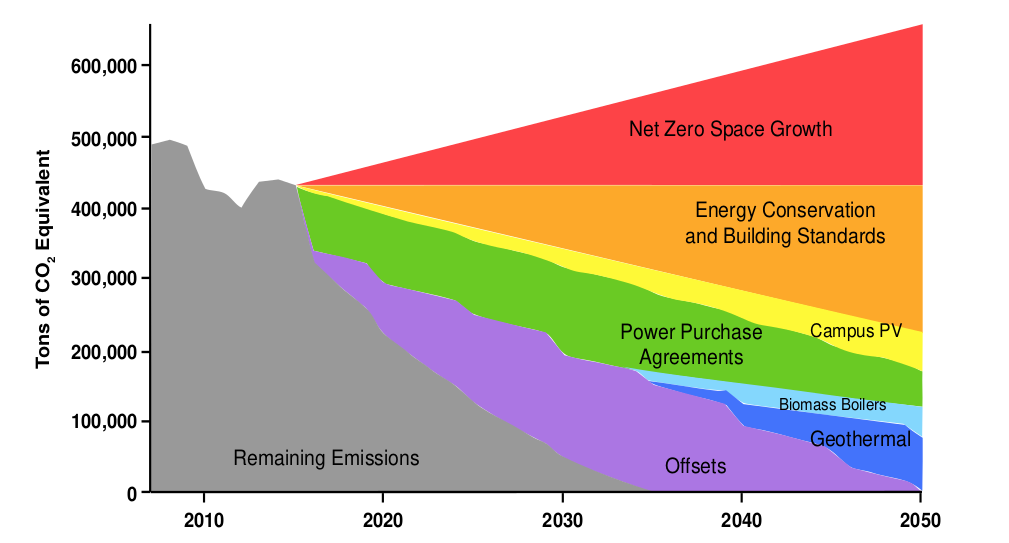
\includegraphics[width=\textwidth]{icap_uiucemissions.png}
      \caption{Shows projected CO$_2$ emissions for UIUC \cite{isee_illinois_2015}. Offsets include shutdown of the Blue Waters Supercomputer.}
      \label{fig:co2projections}
    \end{figure}

    \column[t]{5cm}
    \textbf{Goal}:\\
    Carbon neutrality by 2050 or sooner.\\
    \vspace{1cm}
    \textbf{Obstacles}:\\
    \begin{enumerate}
      \item Requires \textit{zero net space growth}.
      \item Campus depends on a system of steam tunnels for heating.
      \item and more...
    \end{enumerate}
  \end{columns}
\end{frame}

\subsection{Need for Nuclear}
\begin{frame}
  \frametitle{The Nuclear Option}
  \begin{columns}
    \vspace{0.25cm}
    \column[t]{5cm}
      \textbf{Nuclear energy...}
      \vspace{0.25cm}
      \begin{enumerate}
        \item ...produces almost no carbon emissions \cite{intergovernmental_panel_on_climate_change_climate_2014}.
        \item ...can produce high-temperature steam.
        \item ...requires little physical space$^*$.
      \end{enumerate}
      \vspace{3cm}
      *compared to solar and wind.
    \column[t]{5cm}
    \begin{figure}
      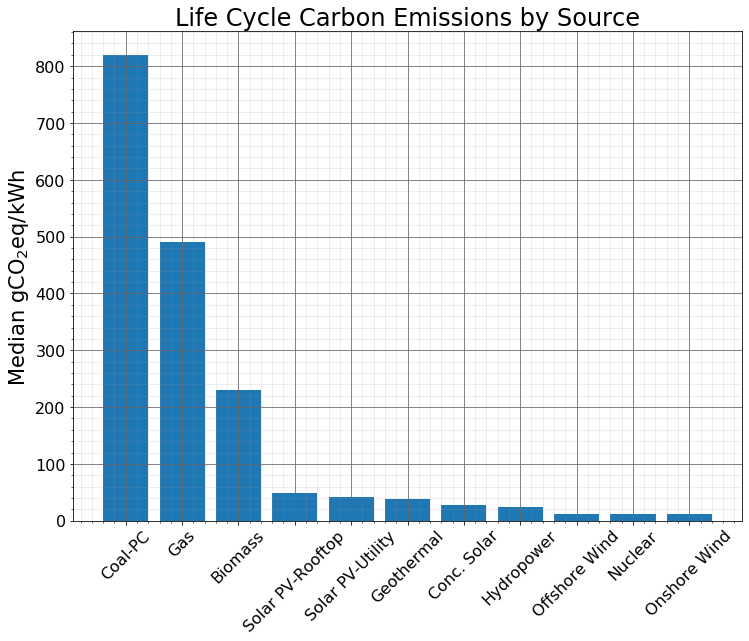
\includegraphics[width=\textwidth]{co2emissions_source.png}
      \caption{Lifetime carbon-equivalent emissions by energy source from IPCC findings \cite{intergovernmental_panel_on_climate_change_climate_2014}.}
      \label{fig:co2source}
    \end{figure}
  \end{columns}
\end{frame}

\subsection{Framing the Question}
\begin{frame}
  \begin{center}
    \Huge{\textbf{What is the optimal size for a nuclear reactor on the UIUC grid?}}
  \end{center}
\end{frame}

% \subsection{Problems}
% \begin{frame}
  \frametitle{Cat Math: Part 1}
  % a comment
        \begin{align}
                x &= y
                \intertext{where}
                x &= \mbox{cats}\\
                y &= \mbox{peculiar}
        \end{align}
\end{frame}

\begin{frame}
\frametitle{Cat Math: Part 2}
        Everything in Beamer is just like in \LaTeX.
        Right down to the theorems.
        \begin{theorem}[Pythagoras] 
                $ a^2 + b^2 = c^2$
        \end{theorem}
        \begin{corollary}
                $ x + y = y + x  $
        \end{corollary}
        \begin{proof}
                $\omega +\phi = \epsilon $
        \end{proof}


\end{frame}

\section{Methods}
\input{Methods}
% \subsection{RAVEN}
% \subsection{TEMOA}

\section{Results}
\subsection{RAVEN results}
\begin{frame}
  \frametitle{Step 1: Generate Synthetic Histories}
    \begin{figure}
      \centering
      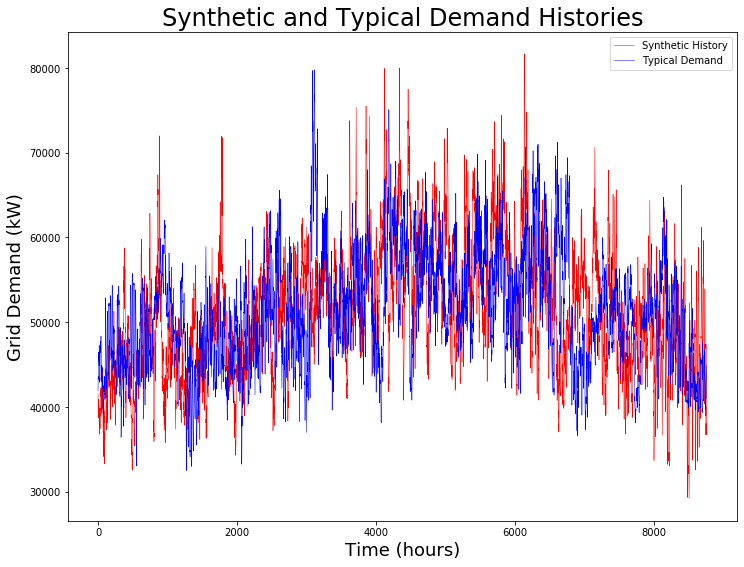
\includegraphics[width=.7\textwidth]{syn_vs_typ_hist.png}
      \caption{Shows the synthetic (red) vs typical (blue) hourly electricity demand at UIUC.}
      \label{fig:syndemand}
    \end{figure}
\end{frame}
\begin{frame}
  \frametitle{Step 1: Generate Synthetic Histories (continued)}
  \begin{figure}
    \centering
    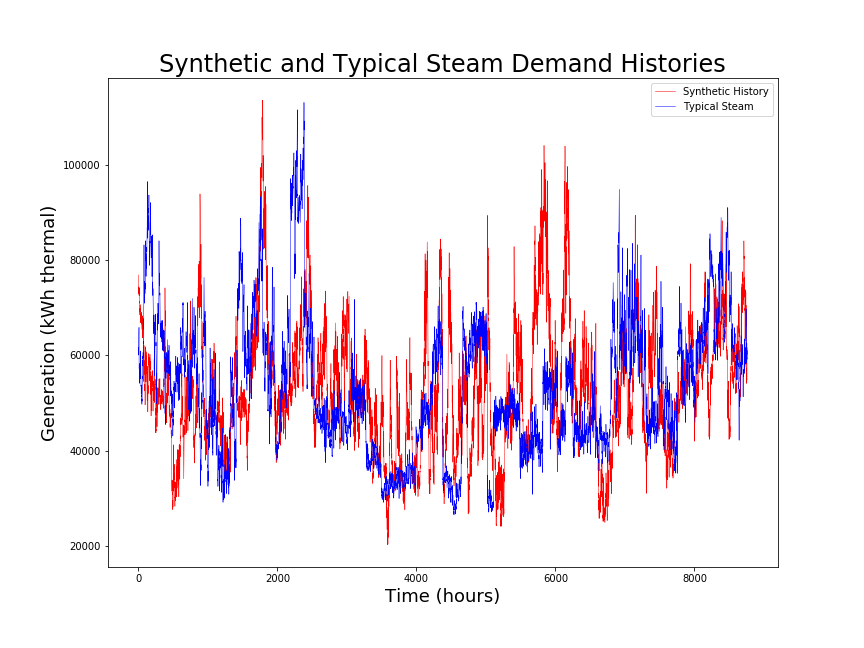
\includegraphics[width=0.7\textwidth]{syn_vs_typ_steam.png}
    \caption{Shows the synthetic (red) vs typical (blue) hourly steam demand at UIUC.}
    \label{fig:synsteam}
  \end{figure}
\end{frame}

\subsection{\texttt{Temoa}: Business As Usual}
\begin{frame}
  \frametitle{BAU: Grid Model}
  \begin{figure}
    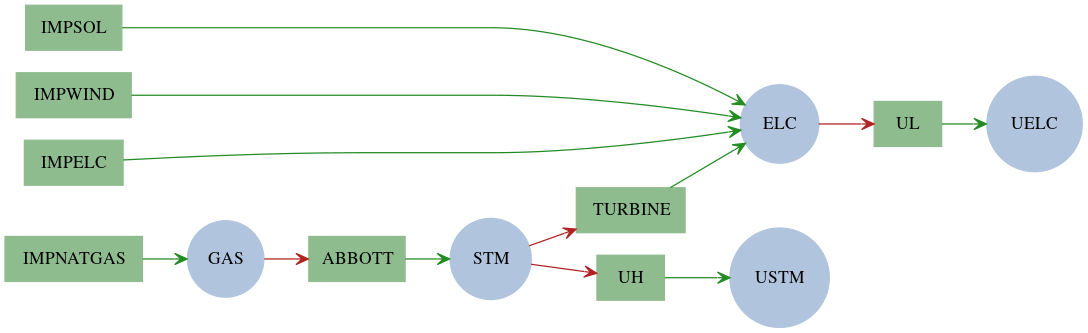
\includegraphics[width=\textwidth]{bau_temoa_uiuc.png}
    \caption{Graph representation of the UIUC embedded grid.}
    \label{fig:uiucgrid}
  \end{figure}
\end{frame}

\begin{frame}
  \frametitle{BAU: Generation}
      \begin{figure}
        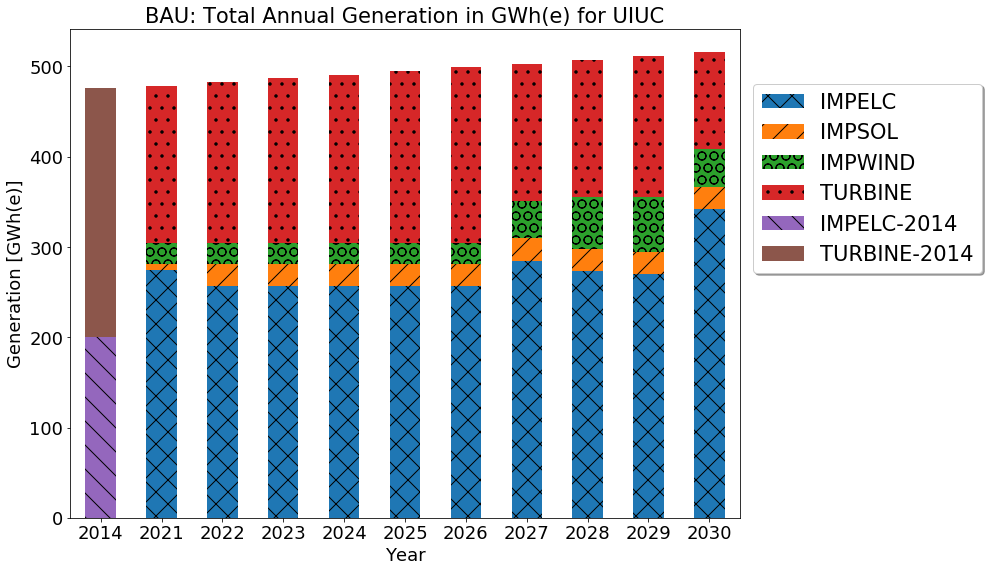
\includegraphics[width=0.8\textwidth]{bau_generation_w2014.png}
        \caption{The change in activity from each energy source from 2020-2030. Assuming 1\% demand growth each year}
        \label{fig:bau_generation}
      \end{figure}

\end{frame}

\begin{frame}
  \frametitle{BAU: Emissions}
  \begin{columns}
    \column[t]{5cm}
      \begin{figure}
        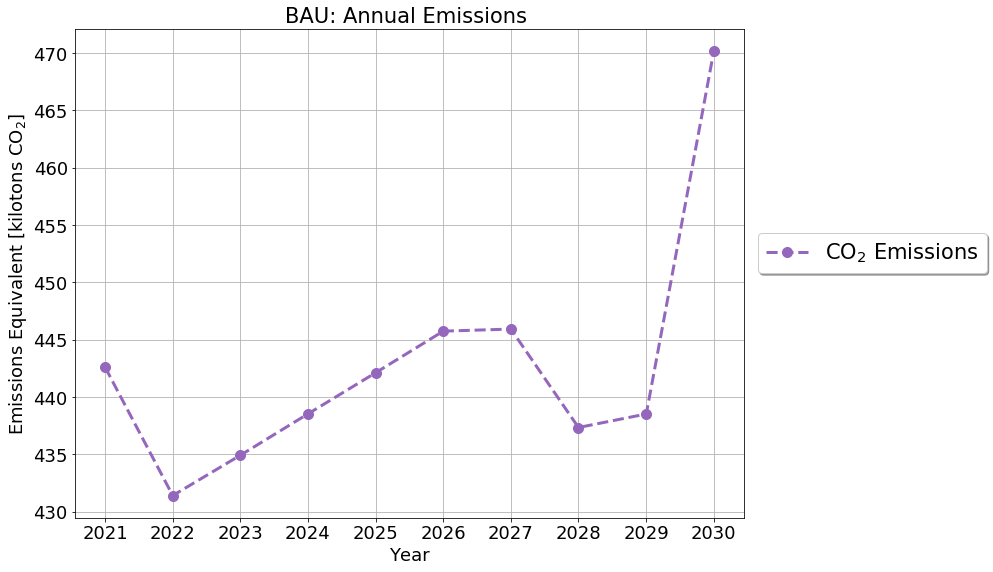
\includegraphics[width=\textwidth]{bau_emissions.png}
        \caption{The change in activity from each energy source from 2020-2030. Assuming 1\% demand growth each year}
        \label{fig:bau_generation}
      \end{figure}
    \column[t]{5cm}
    \begin{figure}
        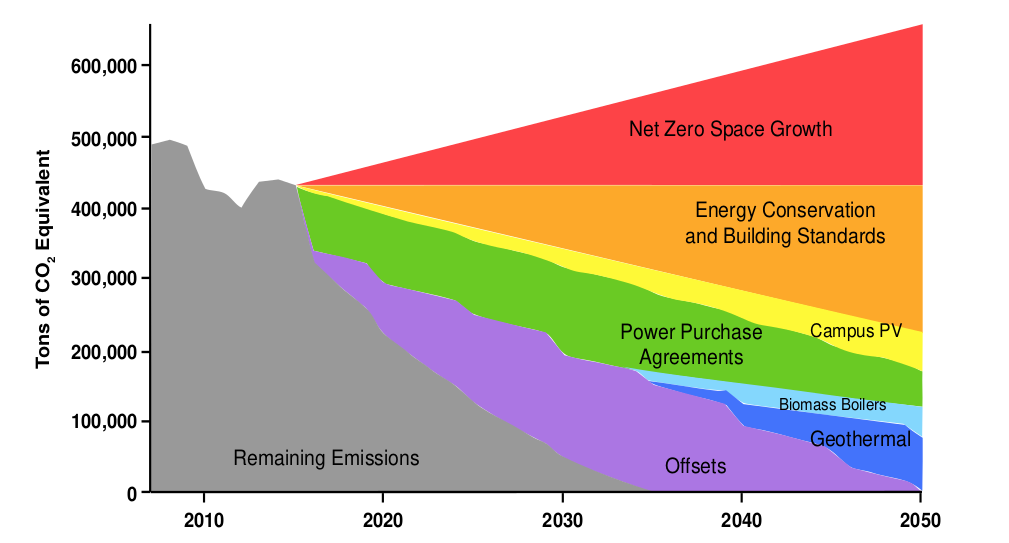
\includegraphics[width=\textwidth]{icap_uiucemissions.png}
        \caption{Predicted growth in emissions from iCAP \cite{isee_illinois_2015}.}
        \label{fig:uiuc_emissions}
      \end{figure}
  \end{columns}
\end{frame}

\subsection{\texttt{Temoa}: Nuclear Scenarios}

\begin{frame}
  \frametitle{Nuclear Scenarios}
  \begin{columns}
    \column[t]{3cm}
    \begin{enumerate}
      \item Scenario 1: Zero Capital Costs
      \item Scenario 2: No Capacity Limit
      \item Scenario 3: Limited to Small Modular Reactor (100MWth)
    \end{enumerate}

    \column[t]{7cm}
    \begin{table}
      \centering
      \caption{Summary of Nuclear Scenarios. Costs from EIA and NEI reports \cite{desai_nuclear_2018}\cite{us_department_of_energy_capital_2016}.}
      \label{table:scenarios}
      \resizebox{\columnwidth}{!}{
      \begin{tabular}{cccc}
        Scenario & Operation Costs & Capital Costs & Maximum Capacity \\
        & [\$/MWh(th)]& [M\$/MWth] & [MWth] \\
        1 & 8.91 & - & - \\
        2 & 8.91 & 1.982 & - \\
        3 & 8.91 & 1.982 & 100 \\
      \end{tabular}
      }
    \end{table}
  \end{columns}
\end{frame}

\begin{frame}
  \frametitle{Nuclear Scenarios: Grid Model}
  \begin{figure}
    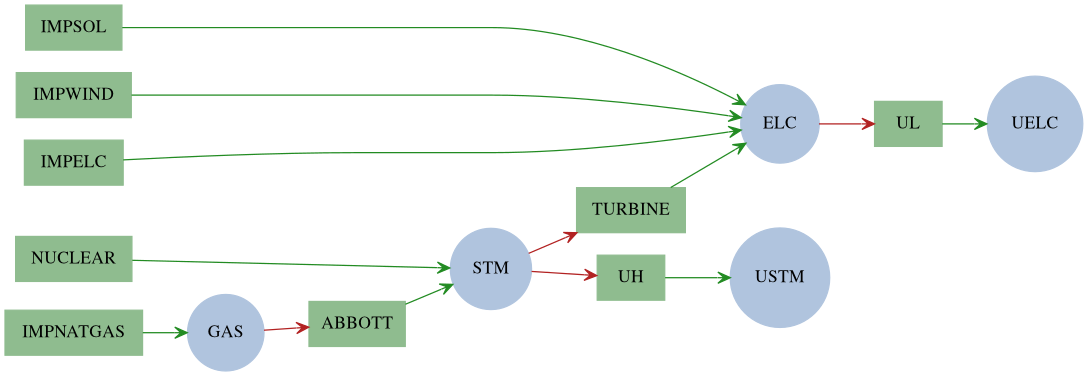
\includegraphics[width=\textwidth]{temoa_uiuc_nuclear.png}
    \caption{Graph representation of the UIUC grid with nuclear reactor.}
    \label{fig:nuclear-uiuc}
  \end{figure}
\end{frame}


\subsection{Scenario 1: Zero Capital Costs}
\begin{frame}
  \frametitle{Scenario 1: Generation}
    \begin{figure}
      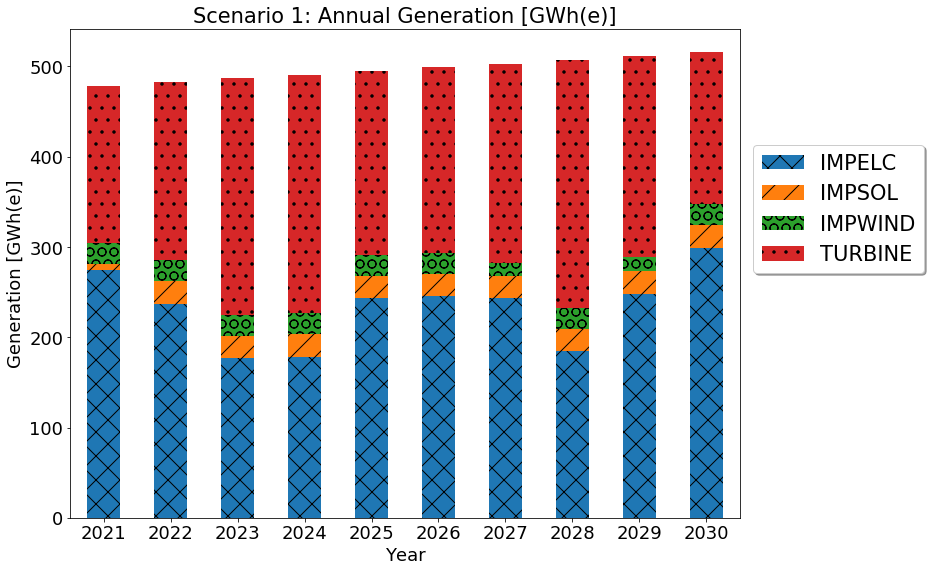
\includegraphics[width=0.9\textwidth]{scenario1_generation.png}
      \caption{The electric generation without a cost constraint on nuclear}
      \label{fig:gen01}
    \end{figure}
\end{frame}
\begin{frame}
  \frametitle{Scenario 1: Emissions}
  \begin{figure}
    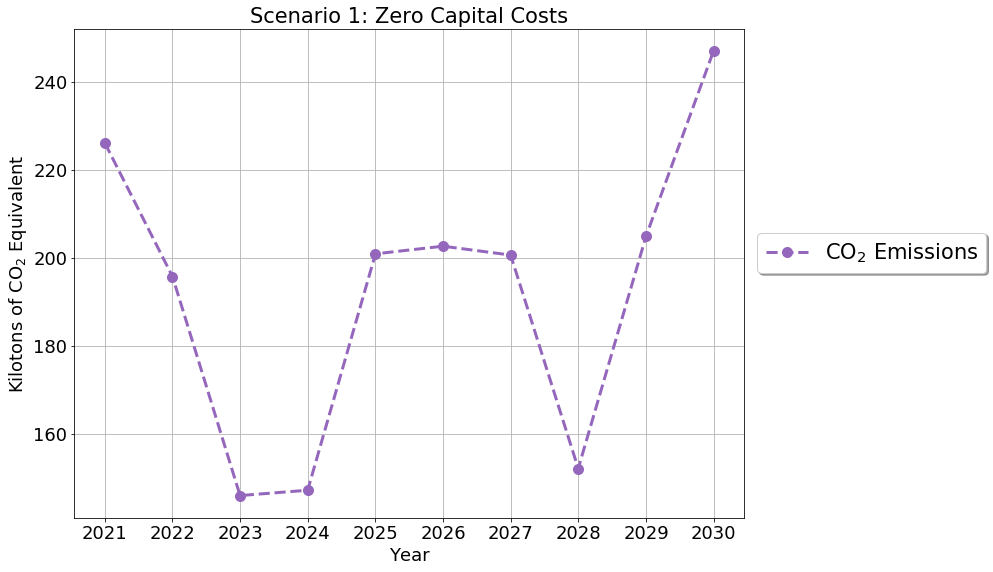
\includegraphics[width=0.9\textwidth]{scenario1_emissions.png}
    \caption{The carbon equivalent emissions without a cost constraint on nuclear}
    \label{fig:emit01}
  \end{figure}
\end{frame}
\subsection{Scenario 2: No Capacity Limit}
\begin{frame}
  \frametitle{Scenario 2: Generation}
  \begin{figure}
    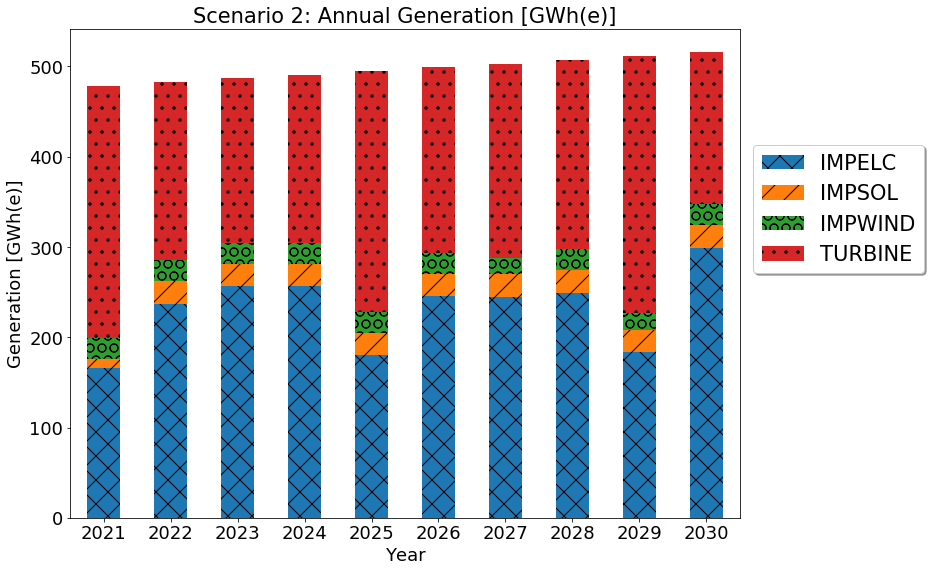
\includegraphics[width=0.9\textwidth]{scenario2_generation.png}
    \caption{The electric generation without a size constraint on nuclear}
    \label{fig:gen02}
  \end{figure}
\end{frame}
\begin{frame}
  \frametitle{Scenario 2: Emissions}
  \begin{figure}
    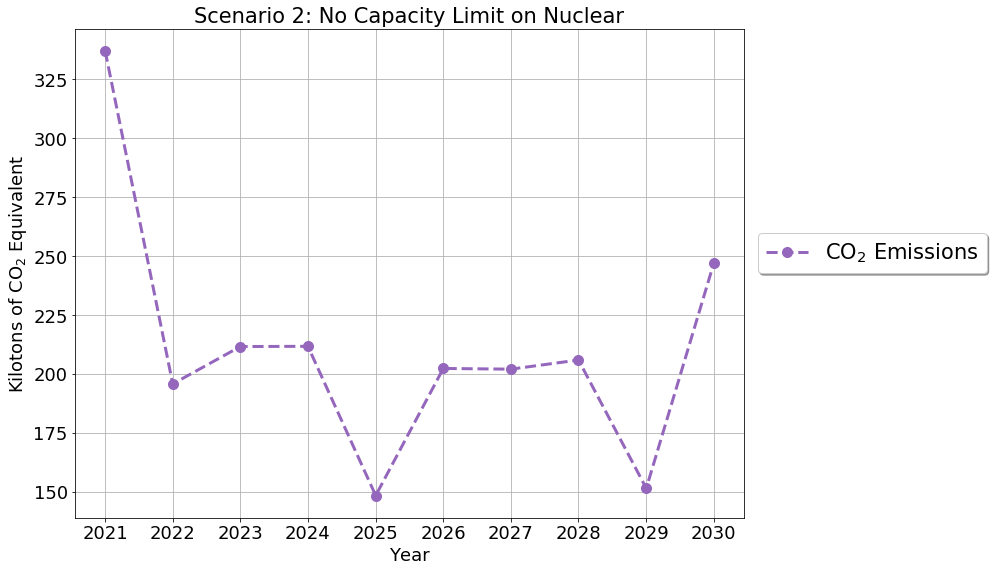
\includegraphics[width=0.9\textwidth]{scenario2_emissions.png}
    \caption{The carbon equivalent emissions without a size constraint on nuclear}
    \label{fig:emit02}
  \end{figure}
\end{frame}
\subsection{Scenario 3: Small Modular Reactor}
\begin{frame}
  \frametitle{Scenario 3: Generation}
  \begin{columns}
    \column[t]{5cm}
    \begin{figure}
      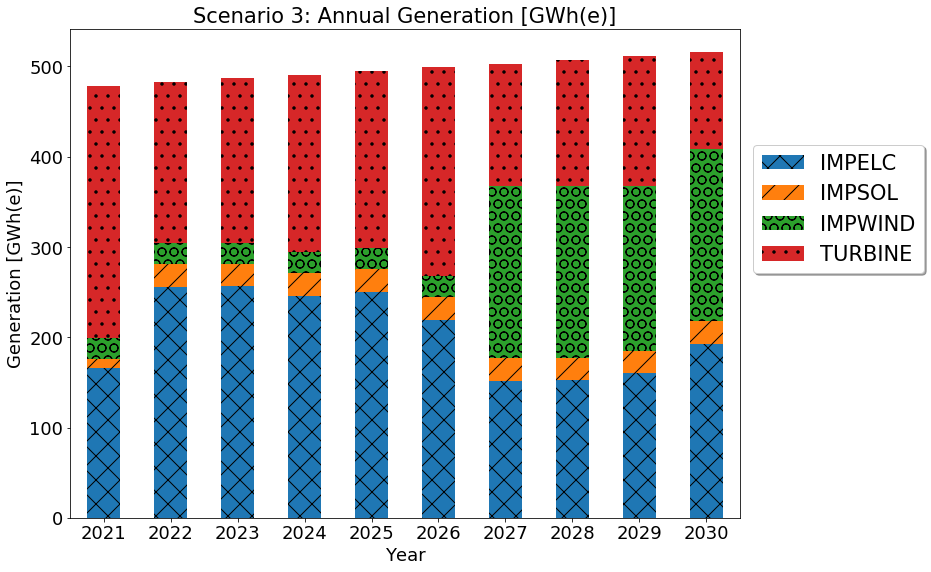
\includegraphics[width=\textwidth]{scenario3_generation_elc.png}
      \caption{The electric generation with constrained nuclear.}
      \label{fig:gen03elc}
    \end{figure}
    \column[t]{5cm}
    \begin{figure}
      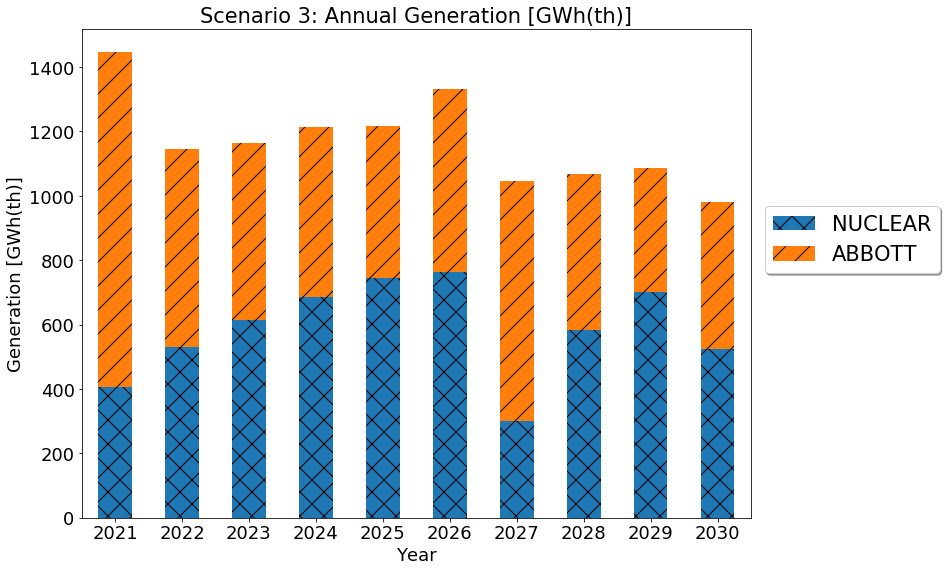
\includegraphics[width=\textwidth]{scenario3_generation_stm.png}
      \caption{The steam generation with constrained nuclear}
      \label{fig:gen02stm}
    \end{figure}
  \end{columns}
\end{frame}
\begin{frame}
  \frametitle{Scenario 3: Emissions}
  \begin{figure}
    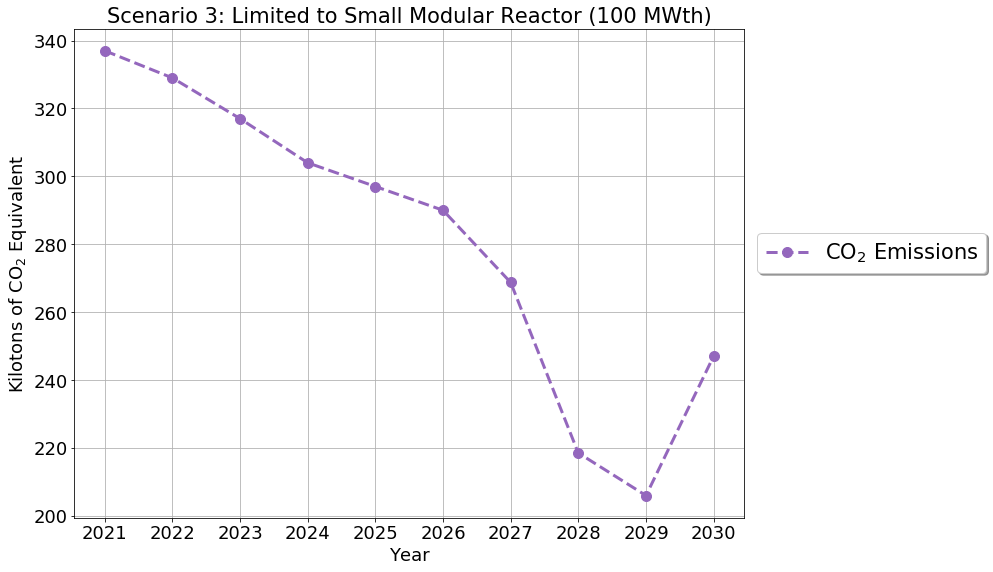
\includegraphics[width=0.9\textwidth]{scenario3_emissions.png}
    \caption{The carbon equivalent emissions without a cost constraint on nuclear}
    \label{fig:emit03}
  \end{figure}
\end{frame}

\section{Conclusion}
\begin{frame}
  \frametitle{Conclusion}
\end{frame}

\begin{frame}
  \frametitle{Acknowledgement}
  This work was made possible with data provided by UIUC Facilities and Services,
  in particular, Morgan White, Mike Marquissee, and Mike Larson. \\
  Also thanks to Roberto Fairhurst and other members of the ARFC group for their
  input.\\
  Additionally, this work is funded by the NRC Fellowship Program. \\
  % Prof. Huff is supported by
  % the Nuclear Regulatory Commission Faculty
  % Development Program (award NRC-HQ-84-14-G-0054 Program B), the Blue Waters
  % sustained-petascale computing project supported by the National Science
  % Foundation (awards OCI-0725070 and ACI-1238993) and the state of Illinois,
  % the DOE ARPA-E MEITNER Program (award DE-AR0000983), the DOE H2@Scale
  % Program (award ), and the International Institute for Carbon Neutral Energy
  % Research (WPI-I2CNER), sponsored by the Japanese Ministry of Education,
  % Culture, Sports, Science and Technology.
\end{frame}

%%--------------------------------%%
%%--------------------------------%%
\begin{frame}[allowframebreaks]
  \frametitle{References}
  \bibliographystyle{plain}
  {\footnotesize \bibliography{bibliography.bib} }

\end{frame}

%%--------------------------------%%


\end{document}
